%% ------------------------------------------------------------------------- %%
\chapter{Desenvolvimento}
\label{cap:desenvolvimento}

Como apresentado na Seção de Introdução, além de existir poucas formas de parametrização de buscas na Web, não há a possibilidade de o usuário ponderar esses parâmetros. Como alternativa, foi desenvolvido o aplicativo \emph{LookingFor}. Esse sistema permite que o usuário ordene os parâmetros da busca de acordo com a sua necessidade. O aplicativo transforma essa ordenação em pesos, que são utilizados na busca parametrizada. Como os resultados não são apenas filtrados, utilizamos os pesos para pontuar os documentos, destacando resultados que podem ser mais relevantes para o usuário.
A estrutura desse aplicativo pode ser vista na figura \ref{fig:diagsis}.

%figura
\begin{figure}[!h]
  \centering
  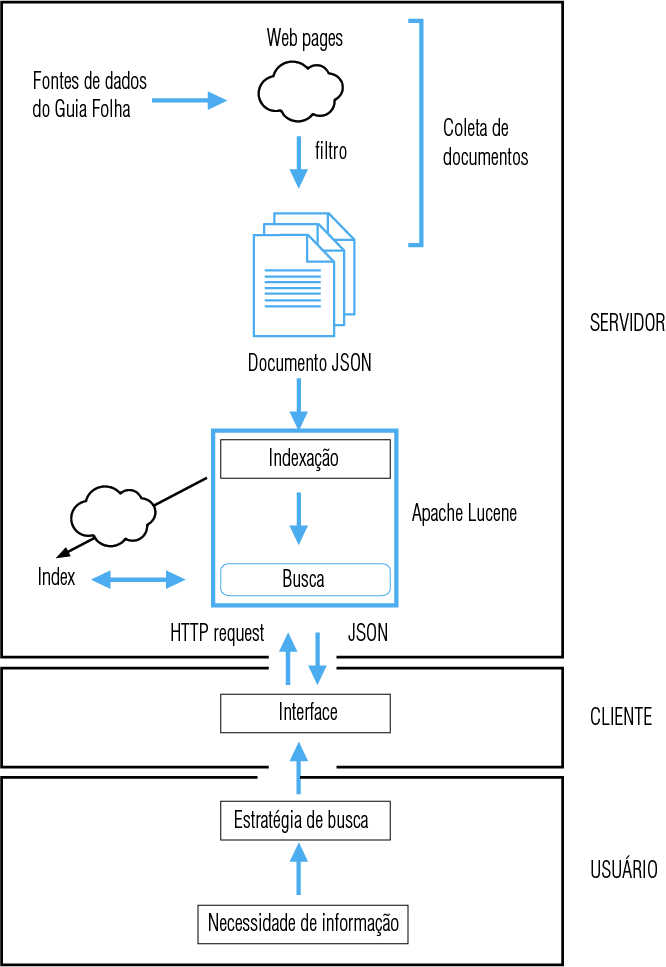
\includegraphics[width=.50\textwidth]{figura_unica.png} 
  \caption{Diagrama do funcionamento do sistema.}
  \label{fig:diagsis} 
\end{figure}

Capturamos documentos HTML da Web e extraímos dados relevantes para as buscas. Para armazenar essas informações, são criados arquivos de metadados. Com a coleção construída, pudemos indexá-la e realizar buscas com auxílio do software open source Apache Lucene \cite{ApacheLucene}. Por fim, os resultados das buscas são apresentados para o usuário através de uma interface.


% %% ------------------------------------------------------------------------- %%
\section{Coleta de documentos e metadados}
\label{sec:coletaDocs}

Para coletarmos documentos, utilizamos um \emph{script Shell} (aplicação criada para interagir com o sistema operacional). Esse \emph{script} acessa e baixa o conteúdo de uma lista de links preestabelecida, gerando documentos locais. Alternativamente, um \emph{Web Crawler} poderia ter sido utilizado nesta etapa. Segundo Manning, Raghavan e Schütze (2008), \emph{Web Crawling} é o processo de coletar páginas da Web, para criar um índice de uma ferramenta de busca. Também é conhecido como indexador automático. Duas alternativas são os softwares livres HTTrack \cite{HTTrack} e Apache Nutch \cite{ApacheNutch}.

% figura
\begin{figure}[!h]
  \centering
  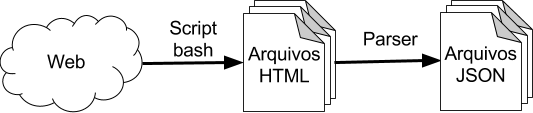
\includegraphics[width=.50\textwidth]{3_2.png} 
  \caption{Diagrama da coleta de documentos da Web.}
  \label{fig:diagcol} 
\end{figure}

A lista de links foi extraída do site Guia Folha \cite{GuiaFolha}. Escolhemos essa fonte, pois suas páginas seguem um padrão de estrutura, contendo dados em \emph{tags} bem definidas do código HTML. 

Após a coleção ter sido criada, executamos uma etapa de limpeza nos documentos HTML. Retiramos todas as \emph{tags} do documento, pois apenas as informações textuais desses documentos têm valor para o usuário. Paralelamente, extraímos dados presentes nos documentos para gerar seus metadados. Para isso utilizamos expressões regulares \cite{ExpRegulares} em partes específicas dos documentos, buscando por conjuntos de caracteres e palavras específicos. Por exemplo, após a expressão ``Telefone:'', uma sequência de dígitos representa o telefone do estabelecimento.

Armazenamos esses metadados no formato JSON (\emph{JavaScript Object Notation}) \cite{JSON}. Utilizamos esse formato por estarmos mais familiarizados. Outras notações poderiam ser utilizadas como o XML (\emph{Extensible Markup Language}) \cite{XML}.

% %% ------------------------------------------------------------------------- %%
\section{Indexação}
\label{sec:indexacao}

Como dito anteriormente, utilizamos o software Apache Lucene \cite{ApacheLucene} para indexar a coleção. O Lucene é uma biblioteca para buscas textuais, sendo amplamente utilizado em sistemas de RI. Possui operações de indexação e busca para coleções de documentos de texto.

A classe \emph{IndexWriter} \cite{IndexWriter} é a responsável por adicionar os documentos ao índice. O índice pode ser armazenado em disco ou em memória, utilizando as classes \emph{FSDirectory} e \emph{RAMDirectory}, respectivamente. Nesta implementação, optamos por guardar o índice no disco, criando novos processos para cada busca.

Para representar os documentos durante a indexação é utilizada a classe \emph{Document}, que armazena suas zonas em objetos da classe \emph{Field}. Dessa forma, é fácil recuperar esses campos individualmente, separando os índices para cada zona que serão a base para a busca parametrizada. Adicionalmente, esses campos podem ser acessados na etapa de busca para atribuir pontuações a dados não-textuais, em que não se aplicam modelos de similaridade como o $tf\textnormal{-}idf$.

Cada documento é processado pela classe \emph{DocConsumer} e armazenado em memória. Essas operações podem ser realizadas por várias threads, cada uma mantendo um índice parcial. Através de um sistema de eventos, a classe \emph{MergePolicy} é chamada para mesclar esses índices parciais ao principal, mantendo sua consistência. A instância da classe \emph{MergePolicy} é única e serve de ponte entre as diferentes threads e o disco, concentrando os acessos em uma só operação. Com isso, não se desperdiça espaço nos blocos transferidos ou tempo de processamento, como visto na seção \textcolor{red}{colocar referência - cap 4}. 

Criamos uma classe adicional \emph{IndexFiles} para encapsular a indexação de uma coleção. Nela, é aberto o diretório em que se encontra a coleção, iterando os documentos para adicioná-los ao índice, utilizando a classe \emph{ndexWriter}. Para cada documento, utilizamos a classe \emph{Field} para representar seu corpo e seus metadados. Três desses campos são: a faixa de preço do restaurante, as suas coordenadas geográficas e a qualidade do restaurante (uma nota atribuída previamente). Esses valores serão utilizados na etapa de busca.

% %% ------------------------------------------------------------------------- %%
\section{Busca parametrizada}
\label{sec:busca_parametrizada}

Buscas parametrizadas nos permitem um refinamento da busca, analisando mais aspectos de um documento. Como visto, podemos fazer buscas em várias zonas ou campos, procurando informações diferentes. A análise de cada zona nos fornece pontuações separadas que compõem uma nota final dada ao documento. Para isso, são utilizados índices paramétricos. Como dito no \textcolor{red}{REFERÊNCIA - capítulo 6}, um índice paramétrico é composto por outros índices, um para cada zona.

Para zonas ou campos com informações puramente textuais, modelos de similaridade como o $tf\textnormal{-}idf$ são utilizados. Obviamente, para campos com outros domínios, esses modelos não se aplicam. Por exemplo, se buscarmos pelo termo ``1992'' e um documento tiver o termo ``1993'', esse documento não terá uma pontuação, pois a frequência do termo ``1992'' é zero.  Em outras palavras, os termos ``1992'' e ``1993'' são considerados diferentes.

Se analisarmos esses termos como números inteiros, entretanto, podemos dar alguma pontuação a esse documento. Ocorrências do termo ``1992'' podem receber a pontuação 1, por estar o mais próximo possível do termo procurado. O documento com o termo ``1993'' receberá uma nota menor, por exemplo, 0,9. Ou seja, podemos utilizar uma função com domínio nos inteiros e imagem no intervalo [0, 1].

Na aplicação \emph{LookingFor}, o usuário pode fazer uma consulta em linguagem natural e configurar três parâmetros: distância, preço e qualidade. Essa configuração é feita sem utilizar palavras ou faixas de valores disponíveis em filtros. Como já foi dito, o usuário fornece ao sistema uma ordem de prioridade para esses parâmetros, tentando comunicar a sua necessidade, como pode ser visto na figura \ref{fig:listprior}. 

%figura
\begin{figure}[!h]
  \centering
  
\includegraphics[width = 0.5\textwidth]{3_3.png} 
  \caption{Lista de prioridades para os parâmetros.}
  \label{fig:listprior} 
\end{figure}

Essa ordem de prioridade será traduzida em pesos, utilizados para ponderar as pontuações das zonas e campos, como na equação \textcolor{red}{REFERÊNCIA DA EQUAÇÃO}:

% formula
\begin{displaymath}
	score(d, q) = \sum_{i = 1}^n p_{i} s_{i}
\end{displaymath}
%
Para isso, definimos o conjunto de parâmetros P, com os parâmetros distância, preço e qualidade:

%formula
\begin{displaymath}
	P = \{dist,\ \textit{pre\c{c}o}, \ qualid\}
\end{displaymath}
%
Através da interface de usuário, é gerado um vetor $v$ sem repetição com até $|P|$ elementos, como na figura \ref{fig:listprior}. Com isso, definimos o peso do corpo do documento:

%formula
\begin{displaymath}
	p_{corpo} = 1 + |v|
\end{displaymath}
%
E os pesos dos parâmetros:

%formula
\begin{displaymath}
	p_{v[j]} = p_{corpo} - j
\end{displaymath}
%
Utilizando o exemplo da figura \ref{fig:listprior}, os valores dos pesos seriam: $p_{corpo}=3$, $p_{dist}=2$, $p_{\textit{\scriptsize pre\c{c}o}}=1$ e $p_{qualid}=0$. Podemos também normalizar os pesos, de forma que:

%formula
\begin{displaymath}
	\sum_{i} p_{i} = 1
\end{displaymath}

Como utilizamos o modelo saco-de-palavras, e considerando a consulta como um pequeno documento, a pontuação representa a similaridade entre a consulta e o documento que está sendo avaliado. Os parâmetros, no entanto, não são definidos pelo usuário, mas por valores hipotéticos atribuídos pelo sistema. Os usuários apenas definem o texto da consulta e os pesos desses parâmetros na busca.

Encaramos a consulta como um documento ideal $d’$, o que para o nosso sistema significa um estabelecimento muito próximo do local do usuário, muito barato e com a melhor qualidade possível. Vamos analisar cada um desses parâmetros individualmente.

Para o critério qualidade, utilizamos uma enumeração para criar uma relação de ordem entre os elementos. Em nosso estudo de caso, os elementos são: ``ruim'', ``regular'', ``bom'', ``muito bom'' e ``ótimo''. Portanto, $d’$ tem o maior valor de qualidade dentre esses elementos: ``ótimo''. Quanto menor for o valor para um documento, mais distante estará do ideal e menor será a sua pontuação.

%formula
\begin{displaymath}
	s_{qualid,\ d} = \frac{1}{qualidade(d')}qualidade(d)	
\end{displaymath}

O segundo critério que utilizamos é o preço médio dos estabelecimentos. No nosso estudo de caso, uma tupla de valores monetários estava associada a cada documento. Essa tupla define o intervalo de preços do restaurante. Para simplificar a análise, utilizamos a média desses dois valores para o cálculo da similaridade. O valor de preço médio para o $d’$ é R\$ 0,00, ou seja, é um estabelecimento gratuito. Logo, os estabelecimentos com preços mais baixos terão pontuações melhores.

%formula
\begin{displaymath}
	s_{\textit{pre\c{c}o},\ d} = 1 - \frac{1}{max(\textit{pre\c{c}o}(d_{1}), ..., \textit{pre\c{c}o}(d_{n}))}\textit{pre\c{c}o}(d)
\end{displaymath}

Por fim, para o critério distância, utilizamos coordenadas geográficas. Cada estabelecimento possui um endereço, que foi traduzido em coordenadas na etapa de indexação. Para isso, utilizamos a API do GoogleMaps. Para essas coordenadas, a distância entre dois pontos é calculada sobre o globo terrestre. O documento $d’$ possui as mesmas coordenadas geográficas do usuário, ou seja, ele não precisará se locomover. Os estabelecimentos mais próximos do usuário terão pontuações maiores.

%formula
\begin{displaymath}
	s_{dist,\ d} = 1 - \frac{1}{max(dist\hat{a}ncia(d_{1}, d'), ..., dist\hat{a}ncia(d_{n}, d'))}dist\hat{a}ncia(d, d')
\end{displaymath}

Como fica claro, nenhuma dessas pontuações é atenuada. Deixamos isso para os trabalhos futuros. Por exemplo, usar uma função logarítmica ao invés de uma equação de primeiro grau.

Avaliando cada documento sobre esses critérios, podemos finalmente determinar a pontuação final:

%formula
\begin{displaymath}
	score(d,\ q) = p_{corpo} \left(\sum_{t \in q} tf - idf_{t,d}\right) + \sum_{i \in P} p_{i} s_{i}
\end{displaymath}

Encapsulamos o processo de busca e ranqueamento na classe \emph{SearchFiles}, criada sobre o arcabouço Lucene. Essa classe recebe os parâmetros escolhidos pelo usuário, utiliza a busca do Lucene e calcula a similaridade para cada parâmetro. Por fim, ordena os resultados por esse ranqueamento antes de devolvê-los ao usuário.

%figura
\begin{figure}[!h]
  \centering
  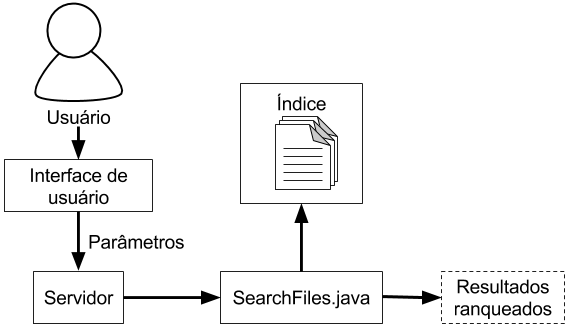
\includegraphics[width=.50\textwidth]{3_4.png} 
  \caption{Diagrama do processamento de uma busca.}
  \label{fig:diagproc} 
\end{figure}

% %% ------------------------------------------------------------------------- %%
\section{Interface de usuário e georreferenciamento}
\label{sec:interface_usuario}

O aplicativo \emph{LookingFor} foi desenvolvido como um sistema Web. A interface de usuário pode ser vista na figura \ref{fig:interfusu}. Ela consiste de três elementos: o formulário de busca, o mapa de georreferenciamento e a lista de resultados. Essas partes podem ser vistas na figura \ref{fig:interfusu}.

A estrutura da consulta é representada no formulário de busca. Ela possui um campo de texto e um botão para cada parâmetro. Ao clicar em um dos botões, um número aparece ao seu lado. Esse número corresponde a prioridade desse parâmetro na busca. Quanto mais baixo o número, maior é o seu peso, como descrito na sessão \ref{sec:busca_parametrizada}. Os parâmetros que não forem escolhidos terão peso zero. Conforme o usuário seleciona e desfaz essas seleções os pesos são ajustados automaticamente por uma função javascript, presente na própria interface.

%figura
\begin{figure}[!h]
  \centering
  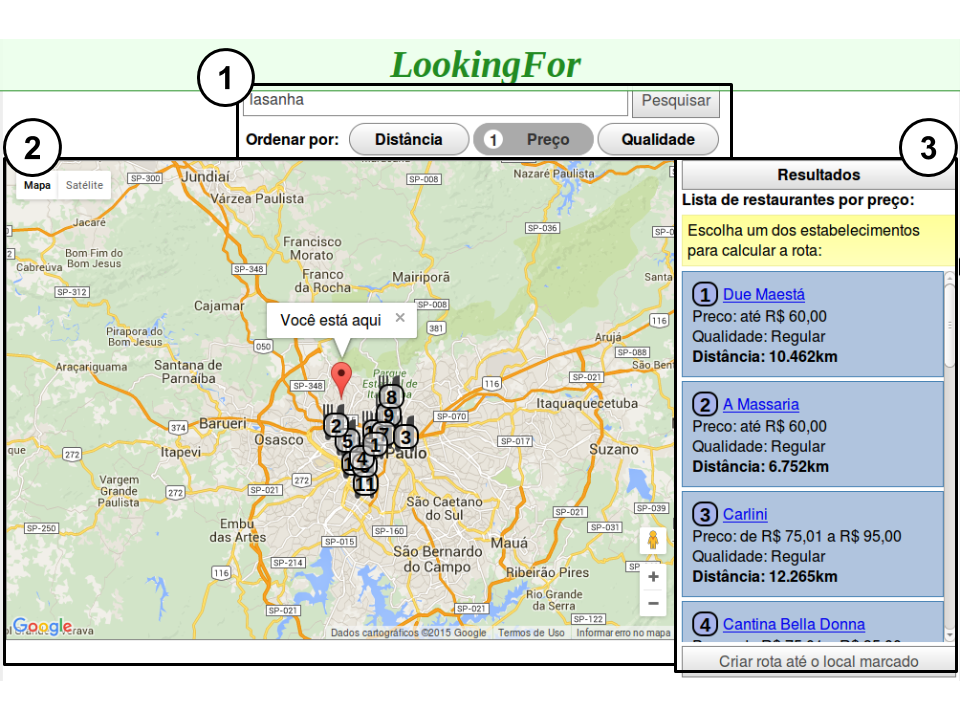
\includegraphics[width=.70\textwidth]{PartesDoSite.png} 
  \caption{Interface do usuário}
  \label{fig:interfusu} 
\end{figure}

Quando o usuário envia o formulário, uma requisição HTTP é feita para o servidor utilizando o padrão AJAX (\emph{Asynchronous Javascript and XML}). A busca é feita no índice e os resultados retornados no formato JSON. Os estabelecimentos são extraídos como objetos javascript e apresentados na lista de resultados à direita na tela. Nessa lista, são apresentadas algumas informações sobre cada estabelecimento: o endereço, a qualidade e a faixa de preço. Dessa forma, o usuário pode entender mais claramente a influência dos parâmetros na busca.

Os resultados também são representados no mapa à esquerda da tela, através do georreferenciamento de seus endereços físicos. Segundo Meireles, Almeida e Silva (2009) ``Georreferenciar é atribuir coordenadas a um ponto de um mapa, vinculando-o a um sistema de coordenadas real.'' O georreferenciamento é utilizado por alguns sistemas para ajudar na compreensão das distâncias entre resultados e sua localização em relação a algum referencial. Essa forma de apresentar os resultados é mais visual, por transformar endereços em pontos em um sistema de coordenadas. 